\documentclass[11pt,a4paper]{article}
\usepackage[margin=2cm]{geometry}
\usepackage{amsmath,amssymb}
\usepackage{tikz}
\usetikzlibrary{positioning,arrows.meta,calc,fit,backgrounds}
\usepackage{booktabs}
\usepackage{array}
\usepackage{xcolor}

\definecolor{classical}{HTML}{2563EB}
\definecolor{quantum}{HTML}{7C3AED}
\definecolor{fusion}{HTML}{059669}
\definecolor{head}{HTML}{DC2626}

\title{\textbf{HybridArielRegressor}\\[4pt]\large Hybrid Classical-Quantum Architecture for Five-Gas Atmospheric Retrieval}
\author{ExoBiome -- HACK-4-SAGES}
\date{March 2026}

\begin{document}
\maketitle

%% ===================================================================
\section{Architecture Overview}
%% ===================================================================

The model predicts five log$_{10}$ volume mixing ratios
$\mathbf{y} = (\log\text{H}_2\text{O},\;\log\text{CO}_2,\;\log\text{CO},\;\log\text{CH}_4,\;\log\text{NH}_3) \in \mathbb{R}^5$
from a 52-bin transmission spectrum (4 channels) and 8 auxiliary planetary/stellar features.

\begin{equation}
\hat{\mathbf{y}} = \underbrace{h_{\mathrm{cls}}(\mathbf{z})}_{\text{classical head}}
+ \alpha\;\underbrace{\tanh(\boldsymbol{g})}_{\text{gate}}
\;\odot\; \underbrace{h_{\mathrm{qnt}}\!\bigl([\mathbf{z}\,\|\,\text{QC}(\boldsymbol{\theta},\,\pi_\phi(\mathbf{f}))]\bigr)}_{\text{quantum correction}}
\end{equation}

where $\mathbf{z}=[\mathbf{f}\,\|\,\mathbf{s}\,\|\,\mathbf{a}]$ is the concatenated context (256-dim),
$\alpha \in [0,1]$ is a training-schedule ramp, and $\boldsymbol{g}\in\mathbb{R}^5$ is a learnable gate.

%% ===================================================================
\section{Module Specifications}
%% ===================================================================

%% -------------------------------------------------------------------
\subsection{Spectral Encoder}
\label{sec:spectral}
%% -------------------------------------------------------------------

\begin{center}
\renewcommand{\arraystretch}{1.15}
\begin{tabular}{l l l}
\toprule
\textbf{Stage} & \textbf{Operation} & \textbf{Output shape} \\
\midrule
Input & $\mathbf{X}\in\mathbb{R}^{B\times 4 \times 52}$ & $(B,\,4,\,52)$ \\
\midrule
\multicolumn{3}{l}{\textit{Stem}} \\
& Conv1d$(4 \to 32,\;k{=}5,\;p{=}2)$ & $(B,\,32,\,52)$ \\
& GroupNorm$(8,\,32)$ $\to$ GELU & $(B,\,32,\,52)$ \\
\midrule
\multicolumn{3}{l}{\textit{Residual Spectral Block 1\;(32$\to$32)}} \\
& Conv1d$(32\to 32,\;k{=}3,\;p{=}1)$ $\to$ GN $\to$ GELU $\to$ Dropout & $(B,\,32,\,52)$ \\
& Conv1d$(32\to 32,\;k{=}3,\;p{=}1)$ $\to$ GN $\to$ $+$ shortcut $\to$ GELU & $(B,\,32,\,52)$ \\
\midrule
\multicolumn{3}{l}{\textit{Residual Spectral Block 2\;(32$\to$64)}} \\
& Conv1d$(32\to 64,\;k{=}3,\;p{=}1)$ $\to$ GN $\to$ GELU $\to$ Dropout & $(B,\,64,\,52)$ \\
& Conv1d$(64\to 64,\;k{=}3,\;p{=}1)$ $\to$ GN $\to$ $+$ shortcut$^*$ $\to$ GELU & $(B,\,64,\,52)$ \\
\midrule
\multicolumn{3}{l}{\textit{Residual Spectral Block 3\;(64$\to$96)}} \\
& Conv1d$(64\to 96,\;k{=}3,\;p{=}1)$ $\to$ GN $\to$ GELU $\to$ Dropout & $(B,\,96,\,52)$ \\
& Conv1d$(96\to 96,\;k{=}3,\;p{=}1)$ $\to$ GN $\to$ $+$ shortcut$^*$ $\to$ GELU & $(B,\,96,\,52)$ \\
\midrule
\multicolumn{3}{l}{\textit{Dual Pooling}} \\
Mean pool & $\bar{\mathbf{x}} = \frac{1}{L}\sum_l \mathbf{x}_l$ & $(B,\,96)$ \\
Attention pool & $\hat{\mathbf{x}} = \sum_l \text{softmax}(\text{scorer}(\mathbf{x}))_l\,\mathbf{x}_l$ & $(B,\,96)$ \\
\midrule
Projection & Linear$(192\to 96)$ $\to$ LayerNorm $\to$ GELU & $(B,\,96)$ \\
\bottomrule
\end{tabular}
\end{center}

\smallskip
\noindent $^*$Shortcut uses Conv1d$(k{=}1)$ when channel dims differ; Identity otherwise.

\paragraph{Spectral Attention Pool.}
\begin{equation}
\text{scorer}(\mathbf{x}) = \text{Conv1d}_{1\times1}\!\bigl(\text{GELU}\bigl(\text{Conv1d}_{1\times1}(96\to 48)\bigr)\bigr)
\quad\Rightarrow\quad
w_l = \frac{\exp(s_l)}{\sum_{l'}\exp(s_{l'})},\quad
\hat{\mathbf{x}} = \sum_l w_l \mathbf{x}_l
\end{equation}

%% -------------------------------------------------------------------
\subsection{Auxiliary Encoder}
%% -------------------------------------------------------------------

\begin{center}
\begin{tabular}{l l l}
\toprule
\textbf{Stage} & \textbf{Operation} & \textbf{Output} \\
\midrule
Input & $\mathbf{a}_{\mathrm{raw}} \in \mathbb{R}^{B\times 8}$ (standardized, log$_{10}$-transformed) & $(B,\,8)$ \\
& Linear$(8\to 32)$ $\to$ GELU $\to$ Dropout & $(B,\,32)$ \\
& Linear$(32\to 32)$ $\to$ GELU & $(B,\,32)$ \\
\bottomrule
\end{tabular}
\end{center}

\noindent Auxiliary features: \texttt{star\_distance}, \texttt{star\_mass\_kg}, \texttt{star\_radius\_m},
\texttt{star\_temperature}, \texttt{planet\_mass\_kg}, \texttt{planet\_orbital\_period},
\texttt{planet\_distance}, \texttt{planet\_surface\_gravity}.

%% -------------------------------------------------------------------
\subsection{Fusion Encoder}
%% -------------------------------------------------------------------

\begin{center}
\begin{tabular}{l l l}
\toprule
\textbf{Stage} & \textbf{Operation} & \textbf{Output} \\
\midrule
Input & $[\mathbf{s}\,\|\,\mathbf{a}]\in\mathbb{R}^{B\times 128}$ \;(spectral$_{96}$ $\oplus$ aux$_{32}$) & $(B,\,128)$ \\
& Linear$(128\to 128)$ $\to$ GELU $\to$ Dropout & $(B,\,128)$ \\
& Linear$(128\to 128)$ $\to$ LayerNorm $\to$ GELU & $(B,\,128)$ \\
\bottomrule
\end{tabular}
\end{center}

%% -------------------------------------------------------------------
\subsection{Regression Heads}
%% -------------------------------------------------------------------

Both the classical and quantum heads share the same \texttt{RegressionHead} template:
\begin{equation}
h(\mathbf{z}) = W_2\,\bigl(\text{Dropout}\bigl(\text{GELU}(W_1\mathbf{z} + b_1)\bigr)\bigr) + b_2
\end{equation}

\begin{center}
\begin{tabular}{l c c c}
\toprule
\textbf{Head} & \textbf{Input dim} & \textbf{Hidden dim} & \textbf{Output dim} \\
\midrule
Classical & 256 & 192 & 5 \\
Quantum & $256 + n_q$ & 192 & 5 \\
\bottomrule
\end{tabular}
\end{center}

\noindent The head context $\mathbf{z}=[\mathbf{f}\,\|\,\mathbf{s}\,\|\,\mathbf{a}]\in\mathbb{R}^{256}$
concatenates fused (128), spectral (96), and auxiliary (32) features.

%% ===================================================================
\section{Quantum Branch}
%% ===================================================================

%% -------------------------------------------------------------------
\subsection{Quantum Projector}
%% -------------------------------------------------------------------

Maps the 128-dim fused representation to $n_q$ rotation angles:
\begin{equation}
\boldsymbol{\theta} = \pi\,\tanh\!\bigl(\text{LN}(W_2(\text{Dropout}(\text{GELU}(W_1\mathbf{f}))))\bigr) \;\in\; [-\pi,\,\pi]^{n_q}
\end{equation}

Default configuration: $n_q = 8$ qubits.

%% -------------------------------------------------------------------
\subsection{Variational Quantum Circuit (QuantumBlock)}
%% -------------------------------------------------------------------

\paragraph{Encoding layer.} Angle embedding with $R_Y$:
\begin{equation}
\text{Encoding:}\quad \prod_{i=0}^{n_q-1} R_Y(\theta_i)\ket{0}^{\otimes n_q}
\end{equation}

\paragraph{Variational blocks} ($B = \texttt{depth}/2$ blocks, default depth$=2 \Rightarrow B=1$).
Each block applies:
\begin{equation}
\underbrace{\prod_{i} R_Y(w_i)}_{\text{rotation}}
\;\to\;
\underbrace{\prod_{i} \text{CNOT}(i,\,(i{+}1)\bmod n_q)}_{\text{entanglement}}
\;\to\;
\underbrace{\prod_{i} R_Z(w_j)}_{\text{phase}}
\;\to\;
\underbrace{\prod_{i} CR_X(w_k;\,i,\,(i{+}1)\bmod n_q)}_{\text{controlled rotation}}
\end{equation}

\paragraph{Measurement.} Expectation values of Pauli-$Z$ on each qubit:
\begin{equation}
\mathbf{q} = \bigl(\langle Z_0\rangle,\;\langle Z_1\rangle,\;\ldots,\;\langle Z_{n_q-1}\rangle\bigr) \;\in\; [-1,1]^{n_q}
\end{equation}

\paragraph{Trainable parameters.} $3\,n_q\,B$ variational weights (default: $3\times 8\times 1 = 24$).
Differentiation: adjoint method via PennyLane Lightning backend.

%% ===================================================================
\section{Hybrid Forward Pass}
%% ===================================================================

\begin{equation}
\boxed{
\hat{\mathbf{y}} = h_{\mathrm{cls}}(\mathbf{z})
+ \alpha\;\tanh(\boldsymbol{g})\odot h_{\mathrm{qnt}}\!\bigl([\mathbf{z}\,\|\,\mathbf{q}]\bigr)
}
\end{equation}

\begin{itemize}
\item $\mathbf{s}=\text{SpectralEncoder}(\mathbf{X})\in\mathbb{R}^{96}$
\item $\mathbf{a}=\text{AuxEncoder}(\mathbf{a}_{\mathrm{raw}})\in\mathbb{R}^{32}$
\item $\mathbf{f}=\text{FusionEncoder}([\mathbf{s}\,\|\,\mathbf{a}])\in\mathbb{R}^{128}$
\item $\mathbf{z}=[\mathbf{f}\,\|\,\mathbf{s}\,\|\,\mathbf{a}]\in\mathbb{R}^{256}$ \quad (head context)
\item $\boldsymbol{\theta}=\text{QuantumProjector}(\mathbf{f})\in[-\pi,\pi]^{n_q}$
\item $\mathbf{q}=\text{QuantumBlock}(\boldsymbol{\theta})\in[-1,1]^{n_q}$
\item $\alpha\in[0,1]$: linear ramp over warmup/ramp epochs
\item $\boldsymbol{g}\in\mathbb{R}^5$: learnable per-target gate (init zeros)
\end{itemize}

%% ===================================================================
\section{Training Schedule}
%% ===================================================================

\begin{center}
\begin{tabular}{l l}
\toprule
\textbf{Parameter} & \textbf{Default} \\
\midrule
Classical LR & $2\times 10^{-3}$ \\
Quantum LR & $8\times 10^{-4}$ \\
Optimizer & AdamW (weight decay $10^{-4}$) \\
Scheduler & ReduceLROnPlateau (factor 0.5, patience 2) \\
Loss & MSE (option: Huber) \\
Gradient clip & $\|\nabla\|_2 \leq 5.0$ \\
Batch size & 64 \\
Quantum warmup & 5 epochs (classical-only) \\
Quantum ramp & 4 epochs ($\alpha: 0\to 1$) \\
Early stopping & patience 6 \\
AMP & bfloat16 / float16 on CUDA \\
\bottomrule
\end{tabular}
\end{center}

%% ===================================================================
\section{Architecture Diagram}
%% ===================================================================

\begin{center}
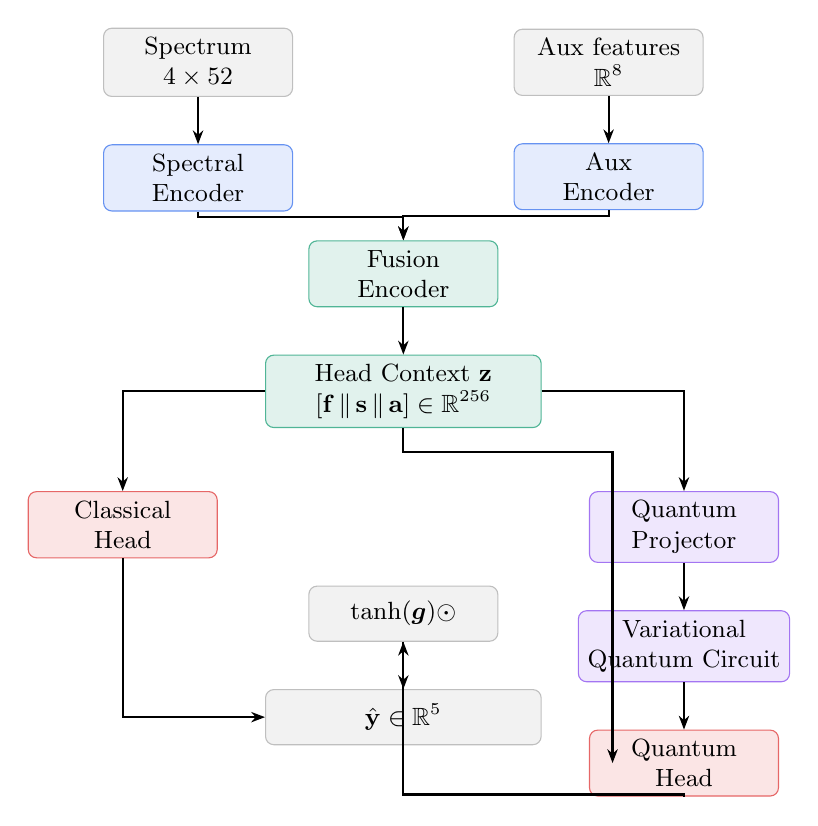
\begin{tikzpicture}[
    node distance=0.6cm and 1.2cm,
    block/.style={draw, rounded corners=3pt, minimum width=2.4cm, minimum height=0.7cm, font=\small, align=center},
    cblock/.style={block, fill=classical!12, draw=classical!70},
    qblock/.style={block, fill=quantum!12, draw=quantum!70},
    fblock/.style={block, fill=fusion!12, draw=fusion!70},
    hblock/.style={block, fill=head!12, draw=head!70},
    io/.style={block, fill=gray!10, draw=gray!50},
    arr/.style={-{Stealth[length=5pt]}, thick},
]
% Inputs
\node[io] (spec_in) {Spectrum\\$4\times52$};
\node[io, right=2.8cm of spec_in] (aux_in) {Aux features\\$\mathbb{R}^8$};

% Encoders
\node[cblock, below=of spec_in] (spec_enc) {Spectral\\Encoder};
\node[cblock, below=of aux_in] (aux_enc) {Aux\\Encoder};

% Fusion
\node[fblock, below=0.8cm of $(spec_enc)!0.5!(aux_enc)$] (fusion) {Fusion\\Encoder};

% Context
\node[fblock, below=of fusion, minimum width=3.5cm] (ctx) {Head Context $\mathbf{z}$\\$[\mathbf{f}\,\|\,\mathbf{s}\,\|\,\mathbf{a}]\in\mathbb{R}^{256}$};

% Classical head
\node[hblock, below left=0.8cm and 0.6cm of ctx] (cls_head) {Classical\\Head};

% Quantum branch
\node[qblock, below right=0.8cm and 0.6cm of ctx] (proj) {Quantum\\Projector};
\node[qblock, below=of proj] (qc) {Variational\\Quantum Circuit};
\node[hblock, below=of qc] (qnt_head) {Quantum\\Head};

% Gate + output
\node[io, below=2.0cm of ctx] (gate) {$\tanh(\boldsymbol{g})\odot$};
\node[io, below=0.6cm of gate, minimum width=3.5cm] (output) {$\hat{\mathbf{y}}\in\mathbb{R}^5$};

% Arrows
\draw[arr] (spec_in) -- (spec_enc);
\draw[arr] (aux_in) -- (aux_enc);
\draw[arr] (spec_enc) -- ++(0,-0.5) -| (fusion);
\draw[arr] (aux_enc) -- ++(0,-0.5) -| (fusion);
\draw[arr] (fusion) -- (ctx);
\draw[arr] (ctx) -| (cls_head);
\draw[arr] (ctx) -| (proj);
\draw[arr] (proj) -- (qc);
\draw[arr] (qc) -- (qnt_head);
\draw[arr] (ctx.south) -- ++(0,-0.3) -| ([xshift=0.3cm]qnt_head.west);
\draw[arr] (cls_head) |- (output);
\draw[arr] (qnt_head) -- ++(0,-0.4) -| (gate);
\draw[arr] (gate) -- (output);
\end{tikzpicture}
\end{center}

%% ===================================================================
\section{Parameter Count Summary}
%% ===================================================================

\begin{center}
\begin{tabular}{l r l}
\toprule
\textbf{Module} & \textbf{Parameters} & \textbf{Group} \\
\midrule
Spectral Encoder (stem + 3 RSB + pool + proj) & ${\sim}52\text{k}$ & Backbone \\
Auxiliary Encoder & ${\sim}1.3\text{k}$ & Backbone \\
Fusion Encoder & ${\sim}33\text{k}$ & Backbone \\
Classical Head & ${\sim}50\text{k}$ & Backbone \\
\midrule
Quantum Projector & ${\sim}17\text{k}$ & Quantum adapter \\
Quantum Gate $\boldsymbol{g}$ & $5$ & Quantum adapter \\
Quantum Head & ${\sim}51\text{k}$ & Quantum adapter \\
\midrule
QuantumBlock (variational weights) & $24$ & Quantum circuit \\
\bottomrule
\end{tabular}
\end{center}

\end{document}
